\documentclass[10pt,a4paper]{article}
\usepackage[margin=21mm,headheight=15pt]{geometry}
\usepackage[T1]{fontenc}
\usepackage{lmodern,amsmath,amssymb,tikz,graphicx,hyperref,fancyhdr,enumitem}
\usetikzlibrary{arrows.meta,positioning,calc,decorations.pathmorphing}
\definecolor{ink}{RGB}{20,53,78}
\hypersetup{colorlinks=true,urlcolor=ink,linkcolor=ink}
\setlength{\parindent}{0pt}\setlength{\parskip}{5pt}
\emergencystretch=3em
\pagestyle{fancy}\fancyhf{}\fancyfoot[C]{\thepage}
\renewcommand{\headrulewidth}{.3pt}
\newcommand{\task}[2]{\par\medskip{\color{ink}\Large\bfseries #1. #2}\par\smallskip}
\newcommand{\answer}{\par\smallskip\textbf{Worked reasoning.} }
\setlist[enumerate]{label=\textbf{(\alph*)},leftmargin=7mm,itemsep=7pt}
\begin{document}
\fancyhead[L]{\small Control of Dynamical Systems}
\fancyhead[R]{\small Laboratory 11}
{\color{ink}\LARGE\bfseries Laboratory 11}\par
{\large Sampling can destabilize a continuous-time design}\par
\textbf{Worked solutions -- five integrated problems}\par
{\small\textbf{Evidence boundary.} Original hypothetical scenarios. Derive, calculate and justify decisions; every numerical record is synthetic. Figures are conceptual and not to scale.}
\smallskip\textbf{Shared nominal data.} Plant: $\dot y=-2y+2u$. Nominal digital PI applies $u_k=2(r_k-y_k)+I_k$ before updating $I_{k+1}=I_k+4T_s(r_k-y_k)$. The exact hold and controller update order are part of the model.
\task{1}{A sampled controller connected to a continuous RC circuit}
The physical example is an ideal $10\,{\rm k}\Omega$ resistor and $50\,\mu{\rm F}$ capacitor, with held input voltage $u$ and capacitor voltage $y$. An ideal ADC/DAC pair connects the circuit to a digital PI controller.
\begin{center}\resizebox{\ifdim\width>.98\linewidth.98\linewidth\else\width\fi}{!}{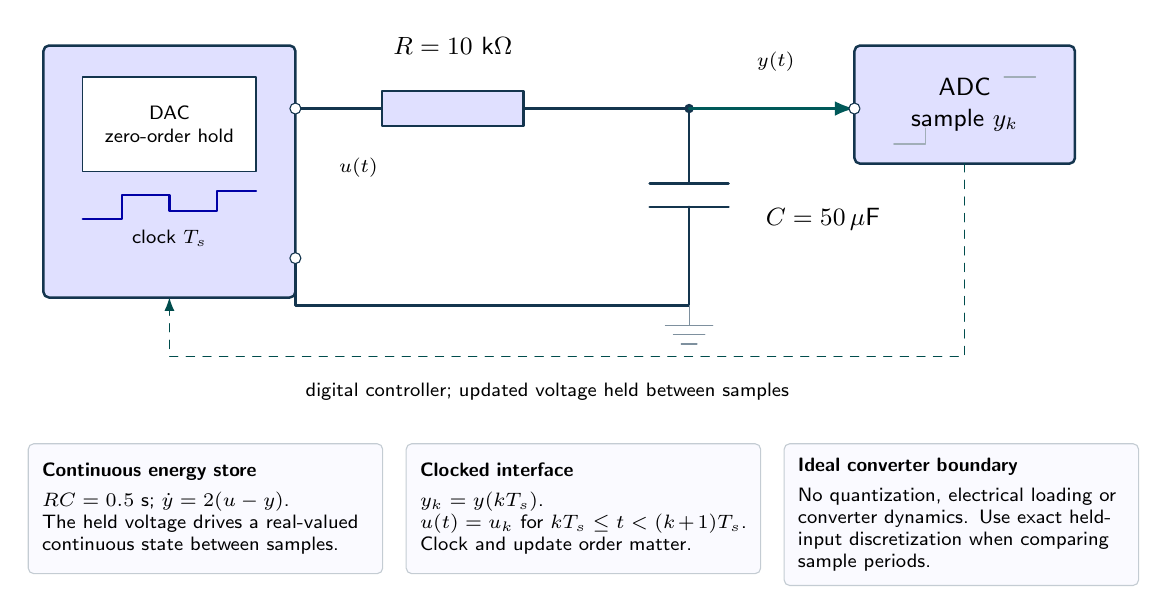
\begin{tikzpicture}[
font=\sffamily\small,>=Latex,line cap=round,line join=round,
wall/.style={draw=ink,line width=1.2pt,fill=blue!5},
water/.style={fill=cyan!25,draw=none},
metal/.style={draw=ink,fill=blue!12,line width=.9pt},
flow/.style={->,draw=blue!65!black,line width=1.2pt},
heat/.style={->,draw=orange!85!black,line width=1.1pt},
measure/.style={->,draw=teal!70!black,line width=.9pt},
dim/.style={<->,draw=ink!65,line width=.6pt},
spring/.style={draw=ink,decorate,decoration={coil,aspect=.5,segment length=4pt,amplitude=3pt}},
wire/.style={draw=ink,line width=1pt},
lab/.style={align=center,font=\sffamily\small},
smalllab/.style={align=center,font=\sffamily\scriptsize}]

\draw[metal,rounded corners=2pt](.2,1)rectangle(3.4,4.2);
\draw[fill=white,draw=ink](.7,2.6)rectangle(2.9,3.8);
\node[smalllab]at(1.8,3.2){DAC\\zero-order hold};
\node[smalllab]at(1.8,1.75){clock $T_s$};
\draw[wire](3.4,3.4)--(4.5,3.4);
\draw[metal](4.5,3.18)rectangle(6.3,3.62);
\draw[wire](6.3,3.4)--(8.4,3.4)--(8.4,2.45);
\draw[wire](7.9,2.45)--(8.9,2.45)(7.9,2.15)--(8.9,2.15);
\draw[wire](8.4,2.15)--(8.4,.9)--(3.4,.9)--(3.4,1.5);
\node[lab]at(5.4,4.2){$R=10$ k$\Omega$};
\node[lab,anchor=west]at(9.25,2.0){$C=50\,\mu$F};
\fill[ink](8.4,3.4)circle(.06);
\draw[measure](8.4,3.4)--(10.5,3.4);
\draw[metal,rounded corners=2pt](10.5,2.7)rectangle(13.3,4.2);
\node[lab]at(11.9,3.45){ADC\\sample $y_k$};
\draw[teal!60!black,dashed,->](11.9,2.7)--(11.9,.25)--(1.8,.25)--(1.8,1);
\node[smalllab]at(6.6,-.2){digital controller; updated voltage held between samples};
\node[smalllab]at(4.2,2.65){$u(t)$};
\node[smalllab]at(9.5,4){$y(t)$};
% REFINED EQUIPMENT DETAILS

% Held waveform, converter terminals and common electrical reference.
\draw[blue!65!black,line width=.8pt](.7,2)--(1.2,2)--(1.2,2.3)--(1.8,2.3)--(1.8,2.1)--(2.4,2.1)--(2.4,2.35)--(2.9,2.35);
\foreach \x/\y in {3.4/3.4,3.4/1.5,10.5/3.4}{\draw[ink,fill=white](\x,\y)circle(.07);}
\draw[ink!55](8.4,.9)--(8.4,.65)(8.1,.65)--(8.7,.65)(8.2,.53)--(8.6,.53)(8.3,.41)--(8.5,.41);
\draw[ink!40](11,2.95)--(11.4,2.95)--(11.4,3.15)(12.4,3.8)--(12.8,3.8);

\node[draw=ink!25,fill=blue!2,rounded corners=2pt,anchor=north west,text width=4.15cm,minimum height=1.65cm,inner sep=5pt,align=left,font=\sffamily\scriptsize]at(0.0,-0.85){\textbf{Continuous energy store}\\[3pt]$RC=0.5$ s; $\dot y=2(u-y)$.\\The held voltage drives a real-valued continuous state between samples.};
\node[draw=ink!25,fill=blue!2,rounded corners=2pt,anchor=north west,text width=4.15cm,minimum height=1.65cm,inner sep=5pt,align=left,font=\sffamily\scriptsize]at(4.8,-0.85){\textbf{Clocked interface}\\[3pt]$y_k=y(kT_s)$.\\$u(t)=u_k$ for $kT_s\leq t<(k+1)T_s$.\\Clock and update order matter.};
\node[draw=ink!25,fill=blue!2,rounded corners=2pt,anchor=north west,text width=4.15cm,minimum height=1.65cm,inner sep=5pt,align=left,font=\sffamily\scriptsize]at(9.6,-0.85){\textbf{Ideal converter boundary}\\[3pt]No quantization, electrical loading or converter dynamics. Use exact held-input discretization when comparing sample periods.};
\end{tikzpicture}
}\par{\small A held voltage drives an ideal RC network. The capacitor voltage is sampled by an ideal ADC; the software controller updates the DAC once per period. Quantization, converter lag and electrical loading are omitted.}\end{center}
\begin{enumerate}
\item The plant is $\dot y=-2y+2u$. Derive its exact update for input held constant over a sampling interval $T_s$, and evaluate coefficients at $T_s=0.5$ s.
\answer Integrating the scalar equation gives $y_{k+1}=e^{-2T_s}y_k+(1-e^{-2T_s})u_k$. Thus $a=e^{-2T_s}$ and $b=1-a$. At 0.5 s, $a=e^{-1}\approx0.367879$ and $b\approx0.632121$. The update is exact at sample instants for held input and this continuous model; it does not approximate the exponential by forward Euler.
\item Use $u_k=2(r_k-y_k)+I_k$ and $I_{k+1}=I_k+4T_s(r_k-y_k)$. Derive the state update matrix for $[y_k,I_k]^T$ and its reference-input vector.
\answer Insert the current integral state into the plant update: $y_{k+1}=(a-2b)y_k+bI_k+2br_k$. The integral update is $I_{k+1}=-4T_sy_k+I_k+4T_sr_k$. Hence $M=\begin{bmatrix}a-2b&b\\-4T_s&1\end{bmatrix}$ and $B_r=[2b,4T_s]^T$. Computing control with $I_{k+1}$ instead of $I_k$ would produce a different matrix and potentially a different stability boundary.
\item Derive the continuous-time PI characteristic polynomial for $k_p=2$, $k_i=4$ and compare its poles with what a sampled implementation must check separately.
\answer The physical circuit has $RC=0.5$ s and $G=1/(0.5s+1)$. With $C=2+4/s$, the characteristic equation is $s(0.5s+1)+2s+4=0$, or $0.5s^2+3s+4=0.5(s+2)(s+4)$. Both continuous poles are stable. Sampling introduces the held-input update and a specific integral-update order; its eigenvalues must lie inside the unit circle. Continuous stability alone imposes no guarantee on an arbitrarily large sampling interval.
\end{enumerate}

\newpage
\task{2}{A stability proof instead of a sampling-rate guess}
Derive the exact sampled characteristic polynomial and apply all second-order Jury conditions. Keep the strictness of the interval explicit.
\begin{enumerate}
\item Derive the characteristic polynomial $z^2-tz+d$ of the update matrix. Express t and d using $a=e^{-2T_s}$.
\answer Since $b=1-a$, the upper-left entry is $3a-2$. Thus $t=\operatorname{tr}M=3a-1$ and $d=\det M=3a-2+4T_s(1-a)$. The polynomial is $z^2-(3a-1)z+[3a-2+4T_s(1-a)]$. Discrete stability requires both root magnitudes below one; negative real parts, the continuous-time criterion, are not sufficient here.
\item Use the real second-order Jury conditions to prove strict stability for $0<T_s<0.75$ and failure for $T_s\ge0.75$. Show the three inequalities rather than only checking selected samples.
\answer For $z^2-tz+d$, the conditions are $1-t+d>0$, $1+t+d>0$ and $1-d>0$. They become $4T_s(1-a)>0$, $6a-2+4T_s(1-a)>0$, and $(1-a)(3-4T_s)>0$. The third gives $T_s<0.75$. For the middle condition, half its value is $f=(3-2T_s)e^{-2T_s}+2T_s-1$. For $0<T_s\le0.5$, the bound $e^{-2T_s}>1-2T_s$ gives $f>2(1-T_s)(1-2T_s)\ge0$. For $0.5\le T_s<0.75$, both terms in f are nonnegative and the exponential term is positive. Thus the exact strict interval is $(0,0.75)$; the third inequality fails afterward.
\item Retain $k_p=2$ but allow positive $k_i$. Derive a necessary sampling bound from the determinant condition alone. Evaluate it at $k_i=8$ and state why the other Jury inequalities are still needed.
\answer Writing $a=e^{-2T_s}$, the determinant becomes $d=3a-2+k_iT_s(1-a)$. Therefore $1-d=(1-a)(3-k_iT_s)>0$ requires $T_s<3/k_i$ for positive $T_s$. At $k_i=8$, this gives $T_s<0.375$ s. It is only one of three strict Jury conditions; the remaining conditions involving $1-t+d$ and $1+t+d$ must also hold. A necessary bound is not automatically a complete stability interval for every gain.
\end{enumerate}

\newpage
\task{3}{The onset of sustained sampled oscillations}
Compare stable, marginal and unstable sample periods. Interpret the boundary in physical time, not only as a point in the discrete z-plane.
\begin{center}\resizebox{\ifdim\width>.98\linewidth.98\linewidth\else\width\fi}{!}{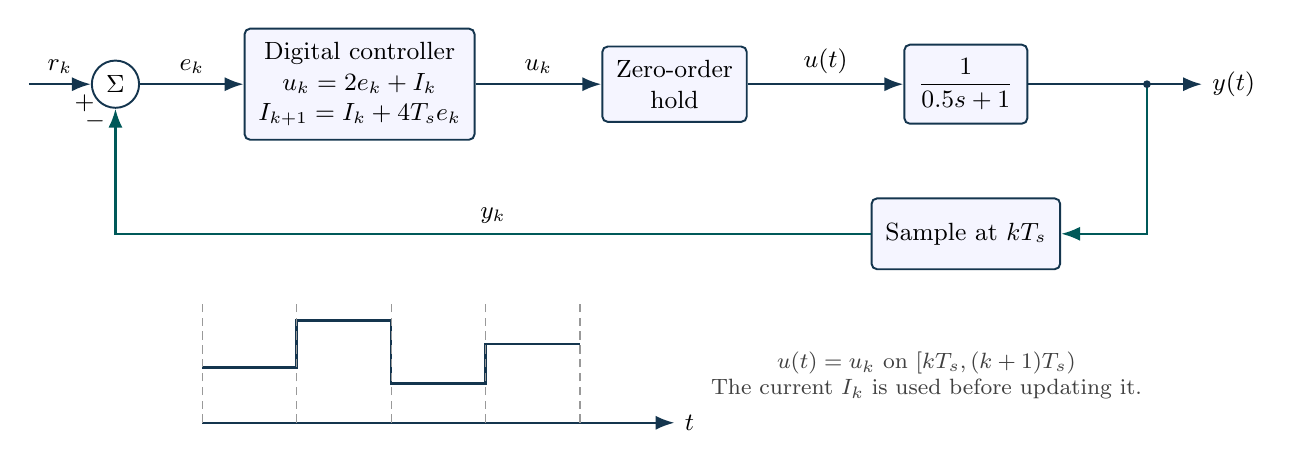
\begin{tikzpicture}[x=1cm,y=1cm,>=Latex,font=\small,
block/.style={draw=ink,fill=blue!4,rounded corners=2pt,minimum height=9mm,align=center,line width=.7pt,inner sep=5pt},
sum/.style={circle,draw=ink,fill=white,minimum size=6mm,inner sep=0pt,line width=.7pt},
sig/.style={->,draw=ink,line width=.85pt},
fb/.style={->,draw=teal!70!black,line width=.85pt},
dist/.style={->,draw=orange!75!black,line width=.85pt},
tap/.style={circle,fill=ink,inner sep=1.4pt},
note/.style={font=\footnotesize,align=center,text=black!75}]

\node[sum](e)at(.9,1.5){$\Sigma$};
\node[block,minimum height=14mm](c)at(4,1.5){Digital controller\\$u_k=2e_k+I_k$\\$I_{k+1}=I_k+4T_se_k$};
\node[block](zoh)at(8,1.5){Zero-order\\hold};
\node[block](p)at(11.7,1.5){$\dfrac{1}{0.5s+1}$};
\draw[sig](-.2,1.5)--node[above]{$r_k$}node[pos=.9,below]{$+$}(e);
\draw[sig](e)--node[above]{$e_k$}(c);
\draw[sig](c)--node[above]{$u_k$}(zoh);
\draw[sig](zoh)--node[above]{$u(t)$}(p);
\draw[sig](p)--(14.7,1.5)node[right]{$y(t)$};
\node[block](sam)at(11.7,-.4){Sample at $kT_s$};
\draw[fb](14,1.5)--(14,-.4)--(sam);
\fill[ink](14,1.5)circle(1.4pt);
\draw[fb](sam)--node[above]{$y_k$}(.9,-.4)--node[pos=.9,left]{$-$}(e);
\draw[sig](2,-2.8)--(8,-2.8)node[right]{$t$};
\draw[line width=1pt,draw=ink](2,-2.1)--(3.2,-2.1)--(3.2,-1.5)--(4.4,-1.5)--(4.4,-2.3)--(5.6,-2.3)--(5.6,-1.8)--(6.8,-1.8);
\foreach \x in{2,3.2,4.4,5.6,6.8}{\draw[black!40,densely dashed](\x,-2.8)--(\x,-1.25);}
\node[note]at(11.2,-2.2){$u(t)=u_k$ on $[kT_s,(k+1)T_s)$\\The current $I_k$ is used before updating it.};

\end{tikzpicture}
}\par{\small The sampler, digital update order and hold are explicit. Continuous plant dynamics and sampled controller states occupy different parts of the loop.}\end{center}
\begin{enumerate}
\item At $T_s=0.75$, find determinant, trace and the nature of the poles. Explain why this endpoint is excluded even though no pole magnitude exceeds one.
\answer Here $a=e^{-1.5}$ and $d=3a-2+3(1-a)=1$. The trace is $t=3e^{-1.5}-1\approx-0.330610$. Since $|t|<2$, the discriminant $t^2-4$ is negative. The conjugate roots have product one, hence each magnitude is one. Generic initial conditions retain an oscillation instead of decaying. Strict asymptotic stability therefore excludes the endpoint.
\item Compute the spectral radius for $T_s=0.05$, 0.5 and 1 s. Classify each implementation and relate the result to the analytic interval.
\answer For each interval form M from Problem 1(b) and take $\rho(M)=\max|\lambda_i(M)|$. The values are approximately 0.893907, 0.606531 and 1.365534. The first two are below one and lie inside the analytic stability interval. The 1 s implementation is unstable. A smaller per-sample radius alone does not compare settling time in seconds because different samples represent different physical durations.
\item At $T_s=0.75$ s, derive the oscillation angle per sample and corresponding angular frequency per second from the conjugate unit-circle pair.
\answer At the boundary, $d=1$ and $t=3e^{-1.5}-1$. Write the roots as $e^{\pm j\psi}$, so $2\cos\psi=t$ and $\psi=\cos^{-1}[(3e^{-1.5}-1)/2]$. The sampled oscillation frequency is $\omega_d=\psi/0.75$ rad/s. The amplitude does not decay for generic excitation of these modes. This frequency belongs to the implemented discrete loop, not to a marginal continuous PI design.
\end{enumerate}

\newpage
\task{4}{An equilibrium is not a convergence guarantee}
The sampled controller has a nominal reference equilibrium even at sample periods that make it unstable. Separate equilibrium equations from local behavior near that equilibrium.
\begin{enumerate}
\item For a mode with discrete magnitude $\rho$, define an equivalent envelope decay rate per second. Compare the two stable sampling periods in Problem 3(b) and explain why this comparison still does not fully describe their transients.
\answer After k samples the envelope is proportional to $\rho^k=e^{(\ln\rho)t/T_s}$. The decay rate is $\gamma=-\ln\rho/T_s$. For 0.05 s it is about 2.243 s$^{-1}$; for 0.5 s it is exactly 1 s$^{-1}$ because $\rho=e^{-1/2}$. Despite the smaller per-sample radius at 0.5 s, its slow envelope decays more slowly in physical time. Pole angles, zeros, initial conditions and intersample behavior also influence the response.
\item For constant reference r and any positive sampling interval, derive the nominal equilibrium of the discrete update. Explain why existence of this equilibrium does not ensure convergence to it.
\answer The integral equation at equilibrium gives $4T_s(r-y)=0$, hence $y=r$. The plant equilibrium satisfies $y=ay+bu$ and $b=1-a>0$, so $u=y=r$. Since proportional error is zero, $I=u=r$. These algebraic values exist even when M is unstable. Convergence depends on its eigenvalues; a generic perturbation grows for $T_s>0.75$ despite the formally correct equilibrium.
\item At $T_s=1$ s and constant $r$, initialize exactly at $[y,I]=[r,r]$. Explain why a perfect simulation can remain there forever although the implementation is unstable, and design a revealing numerical test.
\answer The equilibrium satisfies the update algebraically, so exact arithmetic leaves it unchanged. Stability instead asks whether nearby trajectories return. At $T_s=1$, the spectral radius is about 1.365534, so generic arbitrarily small perturbations grow. Run both the exact-equilibrium case and cases with small state perturbations, report the state-error norm and eigenvalues, and check that roundoff is not being mistaken for a controlled disturbance. An uneventful equilibrium trajectory cannot establish stability.
\end{enumerate}

\newpage
\task{5}{Implementation order and what happens between samples}
Two programs can implement the same displayed PI gains but update the integrator in different orders. Compare the resulting matrices and reconstruct the actual continuous circuit motion.
\begin{enumerate}
\item Now update $I_{k+1}=I_k+4T_s(r_k-y_k)$ first and apply $u_k=2(r_k-y_k)+I_{k+1}$ during the next plant interval. Derive the new matrix and show directly that $T_s=0.5$ is unstable.
\answer Substitution yields $M_{new}=\begin{bmatrix}a-b(2+4T_s)&b\\-4T_s&1\end{bmatrix}$. At $T_s=0.5$, $a=e^{-1}$ and $b=1-a$. Its trace is $5a-3$ and determinant is $3a-2$. The Jury quantity $1+t+d=8a-4$ is negative because $a<1/2$. Hence this implementation is unstable at 0.5 s, although the original update order was stable. Identical gain labels do not specify a digital controller fully.
\item Given $y_k$ and held input $u_k$, derive $y(kT_s+\tau)$ for $0\le\tau\le T_s$. Explain why a plot of sample values alone may conceal an implementation error or performance issue.
\answer The continuous solution within the interval is $y(kT_s+\tau)=e^{-2\tau}y_k+(1-e^{-2\tau})u_k$. At $\tau=T_s$ it must match the exact discrete update. This identity checks held-input simulation and indexing. Sample-only plots omit what happens between samples and may hide an incorrectly applied hold or control-update time. For this scalar first-order plant with constant input, each interval is monotone between its endpoint values; more general plants can have intersample peaks.
\item For this first-order circuit under a truly held input, prove whether an intersample extremum can exceed both endpoint values. Explain why that result does not generalize automatically to a higher-order plant.
\answer Within one hold, $y(kT_s+\tau)=u_k+(y_k-u_k)e^{-2\tau}$. Its derivative is $-2(y_k-u_k)e^{-2\tau}$, whose sign is constant unless it vanishes identically. Thus the ideal first-order trajectory is monotone between samples and cannot have an interior peak beyond both endpoints. Higher-order dynamics, non-held actuation or hidden states can invalidate this property. Sampling-only plots can still hide the wrong update order or an incorrect hold implementation.
\end{enumerate}

\end{document}
